\section{Introduction}
Data are susceptible to various forms of corruption such as missing, incorrect, or inconsistent representations.
Data analysts report that data cleaning is one of the most time consuming steps in the analysis process \cite{nytimes}.
Cleaning can require a significant amount of developer effort in writing software or rules to fix the corruption.
%Crowdsourcing is an increasingly popular alternative, but comes at the cost of additional latency and the overhead of managing human workers \cite{gokhale2014corleone, park2014crowdfill, sampleclean,chu2015katara}.
When data cleaning is expensive, it is desirable to apply it \textbf{progressively}, where analysts can inspect early results with only $k \ll N$ records cleaned.
Progressive data cleaning is a well studied problem especially in the contex of entity resolution \cite{whang2014incremental, papenbrock2015progressive, gruenheid2014incremental}.
Increasingly, Active Learning \cite{settles2010active} or other statistical methods are applied to select records or contraint violations to clean in a way that maximizes the information gained \cite{DBLP:journals/pvldb/YakoutENOI11, gokhale2014corleone, yakout2013don}.

Knowledge of the subsequent data analytics can also help priortize data cleaning.
While this has been explored in the context of conjuctive queries \cite{DBLP:conf/sigmod/BergmanMNT15} and SQL aggregates \cite{wang1999sample}, it is important to recognize the growing popularity of predictive models in data analytics \cite{bdas, alexandrov2014stratosphere, crotty2014tupleware, hellerstein2012madlib}.
Predictive models rely on learning relationships between features and labels, and systematic data corruption \cite{taylor1982introduction} can mask or even introduce spurious new relationships.
Furthermore, the high dimensionality of these models can amplify small problems \cite{xiaofeature} resulting in error-prone predictions even when trained on mostly clean data.

When applied before predictive modeling, straight-forward applications of progressive data cleaning pose several methodological problems.
Suppose $k$ records are cleaned, but all of the remaining dirty records are retained in the dataset.
Training a model on a mixture of dirty and clean data can lead to misleading relationships in even simple scenarios (Figure \ref{update-arch1}).
An alternative is to clean $k$ records and to disregard all of the remaining dirty records (e.g., sampling \cite{wang1999sample}).
While this avoids the mixing problem, accurate model training may require a large amount of training data and $k$ examples may not be enough for a viable model.
Finally, both problems are compounded by sparsity, where if corrupted records are uncommon, a random subset of $k$ records may have relatively few examples of corruptions.
The errors and inefficiencies introduced by these three problems may dominate any gains from data cleaning, leading to unreliable or misleading conclusions about data or model quality.

This paper explores the statistical validity of predictive models when trained on progressively cleaned data.
In particular, we focus on two problems for a popular class of models called convex loss models (e.g., includes linear regression and SVMs): (1) the methodological problem of reliable analysis with progressive data cleaning and predictive modeling, and (2) the algorithmic problem of using information from the model to prioritize data cleaning.
For (1), the key challenge is that predictive model training often implicitly solves an optimization problem and the re-optimization does not commute with progressive data cleaning.
We show that instead of re-optimizing, the model can be incrementally maintained with gradient descent given newly cleaned data, an technique that is guaranteed to converge under suitable conditions.
Such guarantees allow analysts to trust early results during the data exploration and cleaning phase and facilitate reliable comparisons between: expensive data cleaning operations, different types of models, and different featurization techniques.
To address challenge (2), similar to Active Learning, we propose a sampling algorithm that selects the most valuable records to clean with higher probability.
However, an important distinction with prior work is that this prioritization utilizes information from the downstream model.

\begin{figure}[t]
\centering
 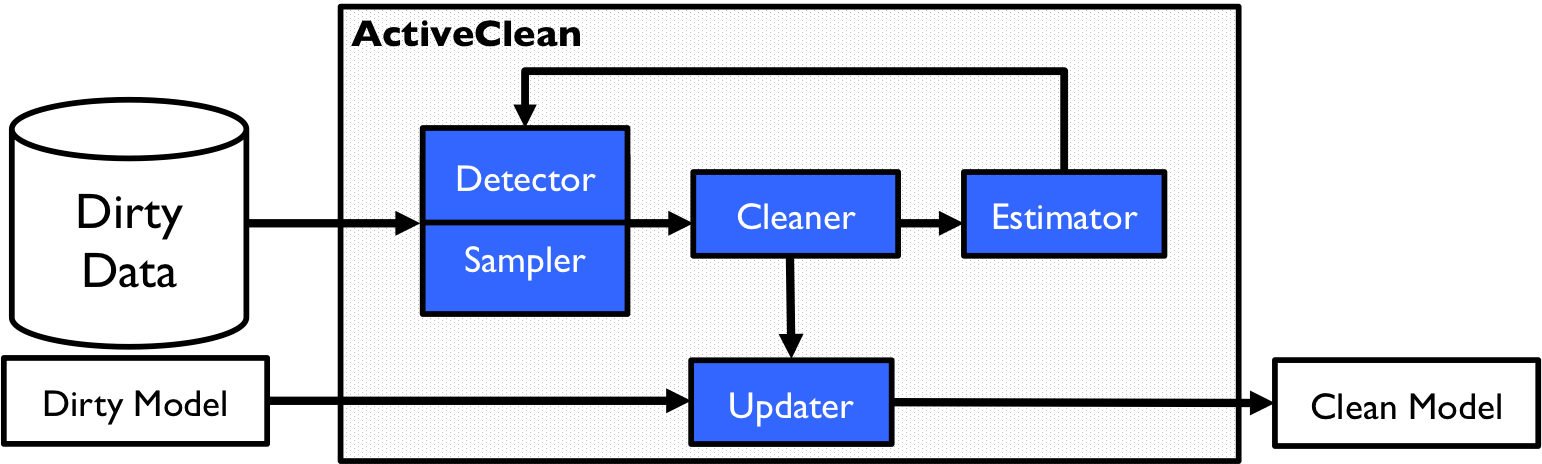
\includegraphics[width=\columnwidth]{figs/arch.png}
 \caption{\sysfull is an architecture where data cleaning is integrated with model training in a framework with sampling, model update, and feedback through estimation. \label{sys-arch}}\vspace{-2em}
\end{figure}

The \sys architecture (Figure \ref{sys-arch}) consists of a \emph{detector}, \emph{sampler}, \emph{cleaner}, \emph{update process}, and \emph{estimator}.
The cleaner is a user-provided data cleaning technique, and \sys provides the remaining components to apply the cleaner progressively.
We analyze a model where the user specifies a cleaning function $C(\cdot)$ where given any record, it returns a cleaned version of the record.
To summarize the contributions by component:
\begin{itemize}[noitemsep]
\item \textbf{Detector} (Section \ref{det}). The detector can apply rules from data quality constraints or adaptively learn which records are dirty to increase the fraction of dirty records sampled.
\item \textbf{Sampler} (Section \ref{dist-samp}). We derive an optimal sampling distribution that minimizes the update variance (i.e., how different would the update be if another sample was drawn) which linearly improves an error bound on the convergence rate.
\item \textbf{Update} (Section \ref{model-update}). The update procedure applies a weighted stochastic gradient descent step to the current best model. This update is guaranteed to converge, and for batch size $b$ and iterations $T$, converges with rate $O(\frac{1}{\sqrt{bT}})$. 
\item \textbf{Estimator} (Section \ref{sampling}). The estimator applies a Taylor Series linearization to decouple changes in different features to use information from error detection to inform estimation.
\item The experiments evaluate these components on four datasets with real and synthetic corruption (Section \ref{eval}). Results suggests that for a fixed cleaning budget, \sys returns more accurate models than uniform sampling and Active Learning when systematic corruption is sparse.

%For a 5\%  systematic corruption, \sys cleans 55\% fewer records to achieve the same accuracy as an Active Learning algorithm.
\end{itemize}






